\section{Versioning Graph}\label{sec:vergraph}

A \textbf{versioning graph} is a linked-data graph which captures the changes separating one version of a data object from another data object.
Utilizing VersOn, the graph between two objects looks like a ladder with the rungs representing the changes affecting the versions as seen in Figure \ref{GCMDC_VerGraph}.
\begin{figure}
	\centering
	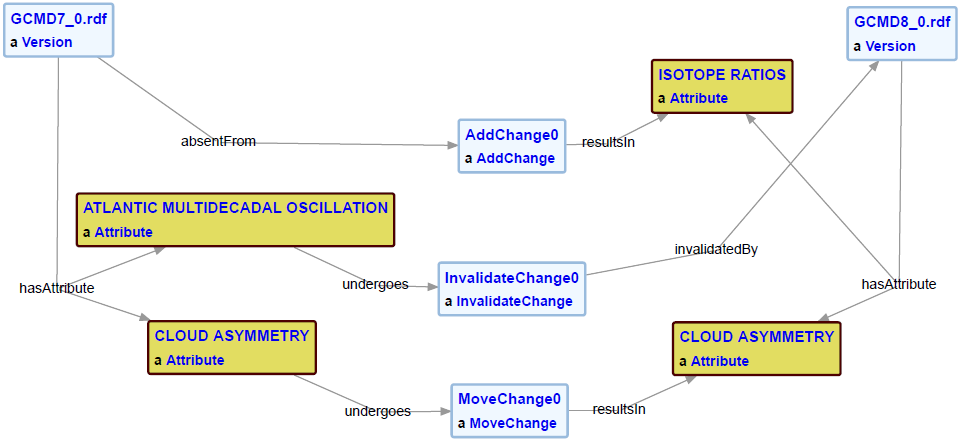
\includegraphics[scale=0.62]{GCMD_VerGraph.png}
	\caption{A sample of the versioning graph between GCMD Versions 7.0 and 8.0, demonstrating an addition, invalidation, and modification.}
	\label{GCMDC_VerGraph}
\end{figure}
The keywords comprise the VersOn Attributes making up the parts of the taxonomy actually changing, in Figure \ref{GCMDC_VerGraph}: `Atlantic Multidecadal Oscillation', `Isotope Ratios', and `Cloud Asymmetry'.
In order to detect the change and the kind of change, we use the unique keyword identifier assigned by the GCMD Keywords group to each keyword.
Since the UUID for each keyword remains the same across versions, the unique keyword identifier can be used to align a mapping across versions.
Additions and invalidations are detected by checking an identifier's presence within both versions.
GCMD Keywords group provides a distribution encoded using SKOS \cite{skos}.
The property \textit{skos:Broader} is used to define the parent term of a keyword in the taxonomy, and we can determine a modification to the taxonomy occurs when a keyword's parent changes.
A difference indicates that the word has been moved to a different place within the taxonomy since identifiers do not change across versions and a keyword only has one parent concept.
The alignment assumes that there is no reason a keyword's preferred label would change, but still reports a value when it has new entries in the ``notes" property.
A change log was generated for each pair of consecutive versions in GCMD Keywords and embedded using JavaScript Object Notation for Linked Data (JSON-LD).
Versioning graphs for each adjacent version were created by extracting JSON-LD from the corresponding change log, and entering the triples into a Fuseki triple store.